\documentclass[table]{beamer}
\usetheme{FAU}
\usefonttheme{FAU}
\usecolortheme{FAU}
\useinnertheme{FAU}
\useoutertheme{FAU}

\usepackage{tikz}
\usepackage{url}
\usepackage{subfigure}

\setbeamerfont{caption}{size=\footnotesize}
\setbeamertemplate{caption}{\raggedright\insertcaption\par}

\newcommand{\goboard}{
	\definecolor{boardcolor}{RGB}{220,179,92}
	\draw [fill=boardcolor,black,thick] (1,1) rectangle (11,11);

	\foreach \x in {0,...,8} {
		\draw[very thick] (2+\x, 2) -- (2+\x, 10) {}; %horizontal
		\draw[very thick] (2, 2+\x) -- (10, 2+\x) {}; %vertikal
	};
}
\newcommand{\piece}[3]{\draw[fill=#1, draw=white!50!black, thick] (#2+1, #3+1) circle (0.5);}
\newcommand{\wpiece}[2]{\piece{white}{#1}{#2}}
\newcommand{\bpiece}[2]{\piece{black}{#1}{#2}}

\title[BT Presentation]{Bachelor Thesis Presentation}
\subtitle{Implementation of an Android app for the recording of Go games by tracking their state}

\institute{Pattern Recognition Lab (CS 5)}

\author{Tilman \textsc{Adler}}
\begin{document}

\frame[plain]{\titlepage}

\frame[squeeze]{\tableofcontents}

\section{Motivation}
\begin{frame}{A Really Short Introduction to Go}

	\begin{columns}
		\begin{column}{0.6\textwidth}
			\begin{itemize}
				\item This is a 9x9 Go board (there's also 11x11, 13x13 and 19x19)
				\visible<2->{\item Players alternately put pieces on the intersections}
				\visible<6->{\item The player with the most area wins}
				\visible<7->{\item \color{gray}Plus: Pieces can be captured, not all moves are allowed}
			\end{itemize}
		\end{column}

		\begin{column}{0.4\textwidth}
			\begin{figure}
				\resizebox{\columnwidth}{\columnwidth}{%
					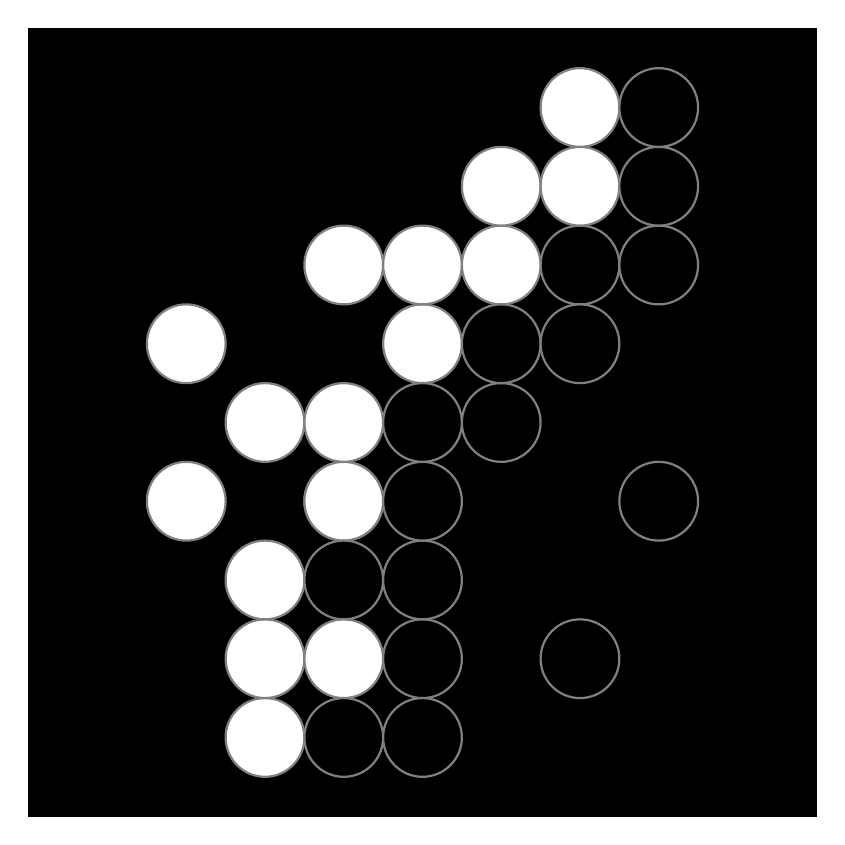
\begin{tikzpicture}[x=1cm, y=1cm]
						\goboard;

						\visible<2->{\wpiece{4}{4};}
						\visible<3->{\bpiece{7}{7};}
						\visible<4->{\wpiece{4}{7};}
						\visible<5->{\bpiece{6}{5};}
						\visible<6->{
							\wpiece{2}{6};\wpiece{2}{4};
							\wpiece{3}{1};\wpiece{3}{2};\wpiece{3}{3};\wpiece{3}{5};
							\wpiece{4}{2};\wpiece{4}{4};\wpiece{4}{5};
							\wpiece{5}{6};\wpiece{5}{7};
							\wpiece{6}{7};\wpiece{6}{8};
							\wpiece{7}{8};\wpiece{7}{9};
							\bpiece{4}{3};\bpiece{4}{1};
							\bpiece{5}{2};\bpiece{5}{3};\bpiece{5}{4};\bpiece{5}{5};\bpiece{5}{1};
							\bpiece{6}{6};
							\bpiece{7}{2};\bpiece{7}{6};
							\bpiece{8}{4};\bpiece{8}{7};\bpiece{8}{8};\bpiece{8}{9};

						}
					\end{tikzpicture}
				}
			\end{figure}
		\end{column}
	\end{columns}
\end{frame}

\begin{frame}{Reasons to Record Go Games}{The famous Ear-reddening Game of 1846}
	\begin{columns}
		\begin{column}{0.6\textwidth}
			\begin{itemize}
				\item This is the game after the 25th move,...
				\visible<2->{\item when black made a mistake, that put white in the lead.}
				\visible<3->{\item The game went on to move 126...}
				\visible<4->{\item when this ingenious move turned the game and let the white player's ears blush. No one but the players noticed what a good move it was.}
			\end{itemize}
		\end{column}
		\begin{column}{0.4\textwidth}
			\begin{figure}
				\only<1>{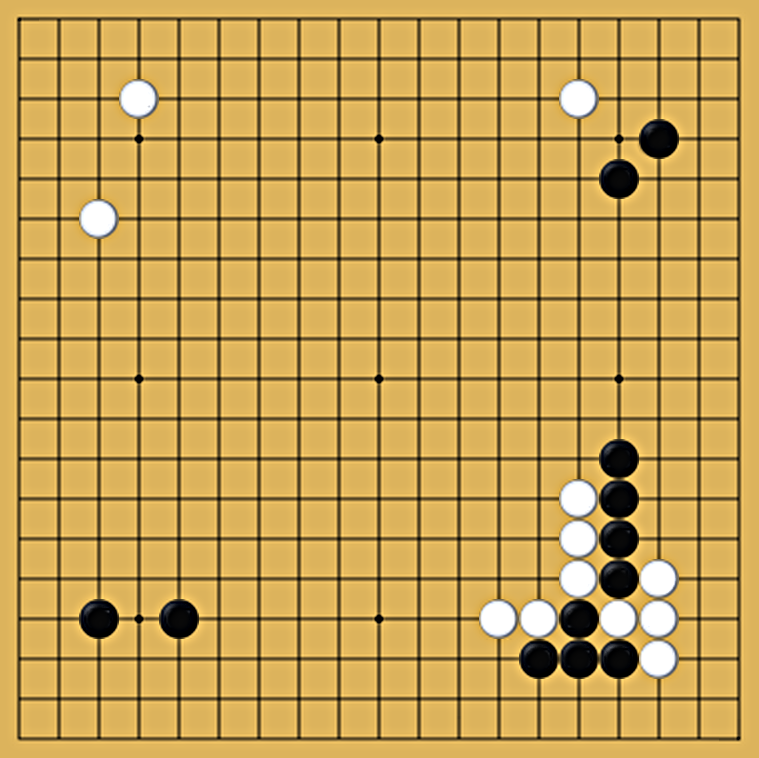
\includegraphics[width=\columnwidth]{images/ear-reddening-24.png}}%
				\only<2>{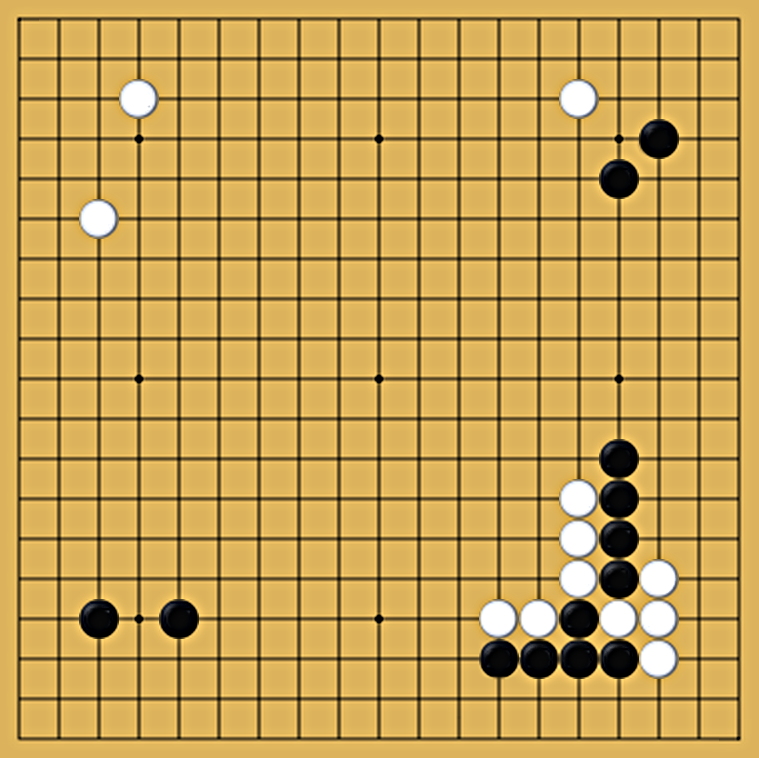
\includegraphics[width=\columnwidth]{images/ear-reddening-25.png}}%
				\only<3>{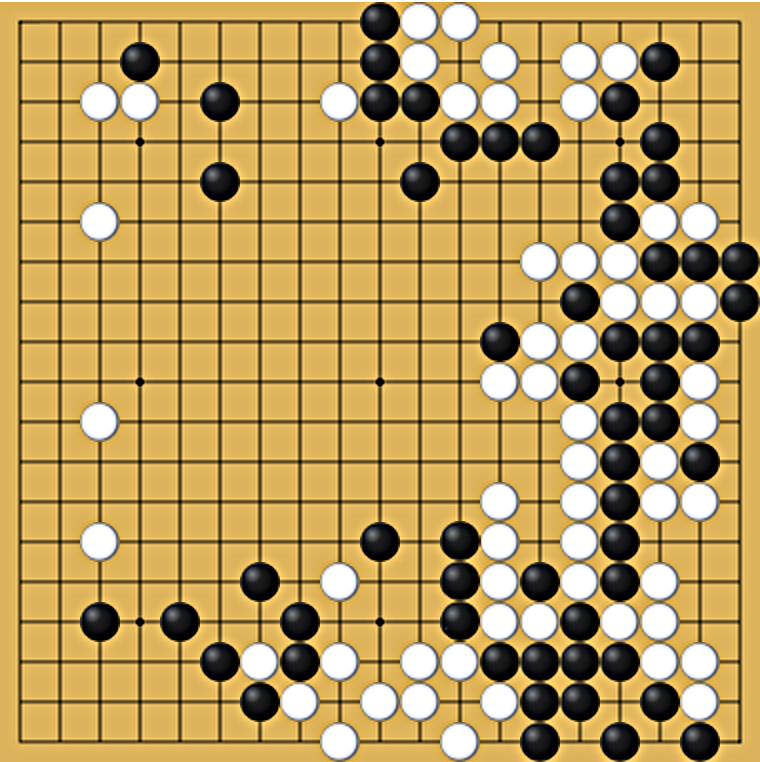
\includegraphics[width=\columnwidth]{images/ear-reddening-126.png}}%
				\only<4>{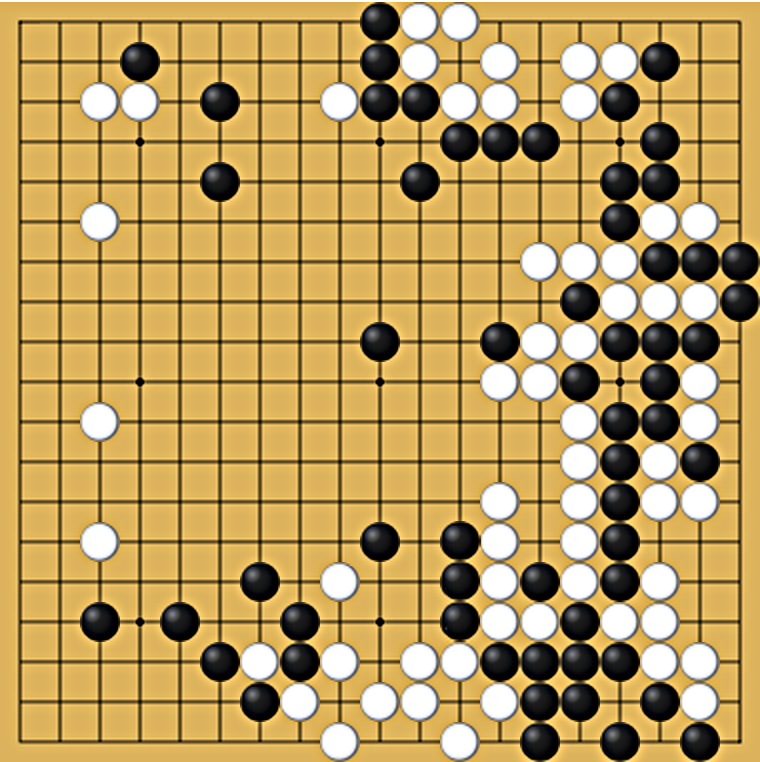
\includegraphics[width=\columnwidth]{images/ear-reddening-127.png}}%
				\caption{\tiny{Image CC-BY-SA 3.0 by Wikipedia \url{http://en.wikipedia.org/w/index.php?title=Ear-reddening_game&oldid=640966258}}}
			\end{figure}
		\end{column}
	\end{columns}
\end{frame}

\section{Detector Pipeline}
\frame[squeeze]{\tableofcontents[currentsection]}

\subsection{Overview}
\begin{frame}{Overview}
	Most of the related work uses only line detection to find the board \\
	$\Rightarrow$ This is problematic for mobile applications\\[0.5cm]

	Our approach is to \begin{itemize}
		\item use line detection for finding intersections
		\item detect pieces, too, for intersections
		\item extrapolate the board from both
		\item classify intersections
	\end{itemize}
\end{frame}

\subsection{Preprocessing}
\begin{frame}{Preprocessing}{Segmenting the board from the background}
	\begin{columns}
		\begin{column}{0.5\textwidth}
			Segmenting the board from the background is useful for
			\begin{itemize}
				\item removal of noisy backgrounds
				\item improving detection speed
			\end{itemize}
			\vspace{0.5cm}
			We use an adaptive threshold and connected-component analysis for this task
		\end{column}

		\begin{column}{0.45\textwidth}
			\only<1>{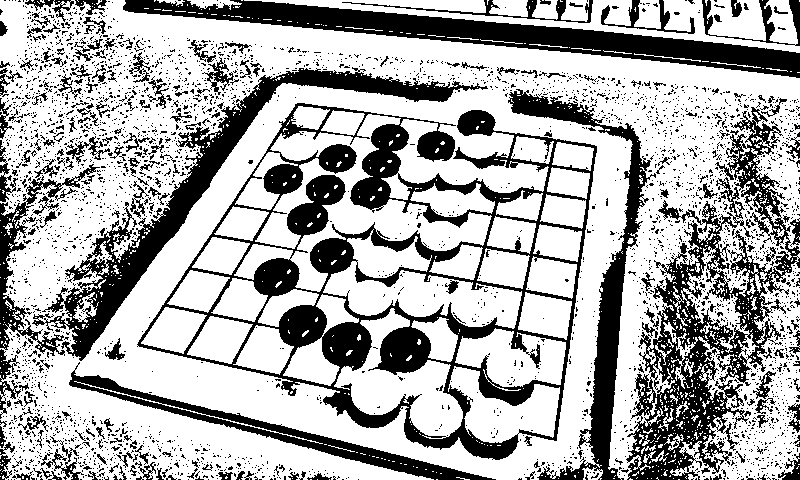
\includegraphics[width=\columnwidth]{images/prep_threshold.png}}%
			\only<2>{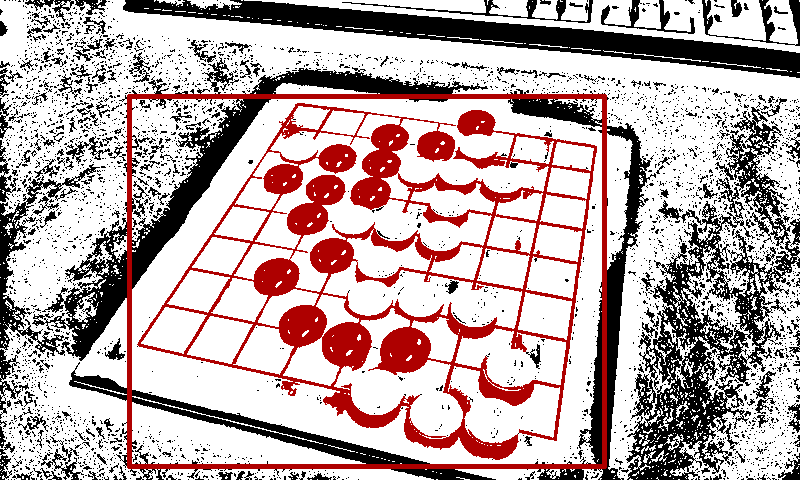
\includegraphics[width=\columnwidth]{images/prep_threshold_1.png}}%
			\only<3>{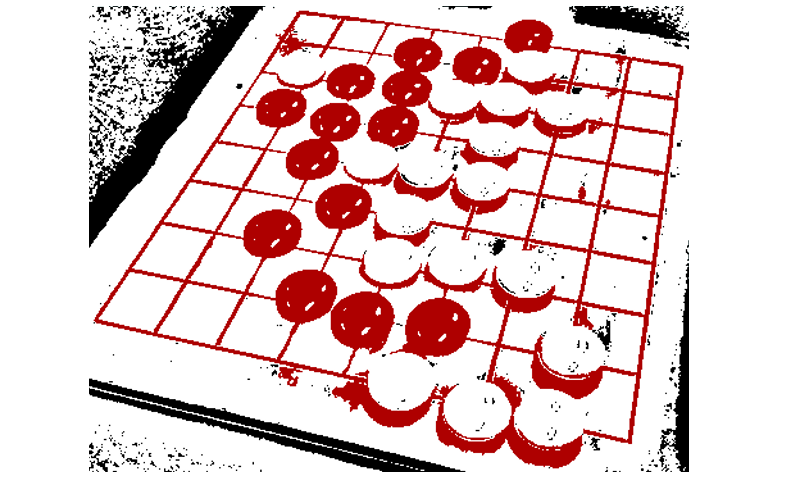
\includegraphics[width=\columnwidth]{images/prep_threshold_2.png}}
		\end{column}
	\end{columns}
\end{frame}

\subsection{Detection of Lines}
\begin{frame}{Detection of Lines}{using Hough Lines Transformation}
	\begin{columns}
		\begin{column}{0.5\textwidth}
			This approach is pretty straight forward:
			\begin{itemize}
				\item detect lines
				\item classify as horizontal/vertical
				\item intersect each horizontal with each vertical
				\item remove duplicates
			\end{itemize}
		\end{column}

		\begin{column}{0.45\textwidth}
			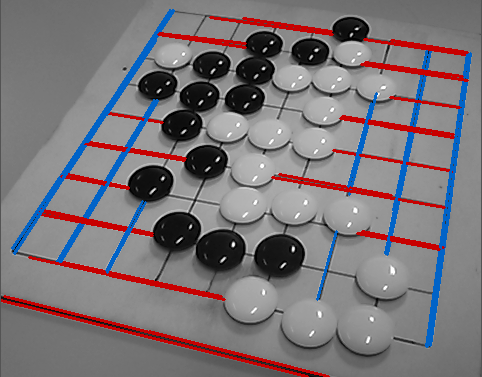
\includegraphics[width=\columnwidth]{images/lineDetection_hough.png}
		\end{column}
	\end{columns}
\end{frame}

\begin{frame}{Detection of Lines}{using the Line Segment Detector}
	\begin{columns}
		\begin{column}{0.45\textwidth}
			Additional steps for \emph{LSD} detector
			\begin{itemize}
				\item filter short lines
				\item filter lines without parallels
				\item stitch lines
			\end{itemize}
		\end{column}
		\begin{column}{0.5\textwidth}
			\begin{figure}
				\begin{center}
					\begin{subfigure}{}
						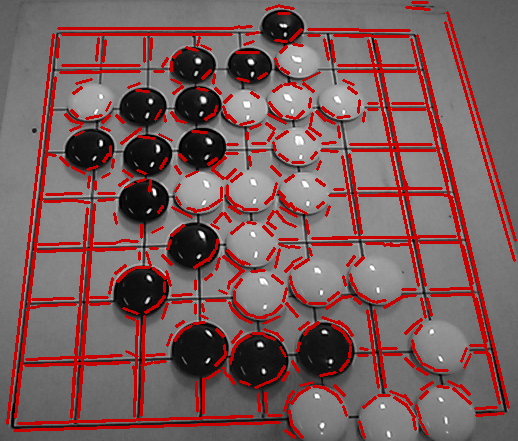
\includegraphics[width=0.45\columnwidth]{images/lsd_first.png}
					\end{subfigure}
					\begin{subfigure}{}
						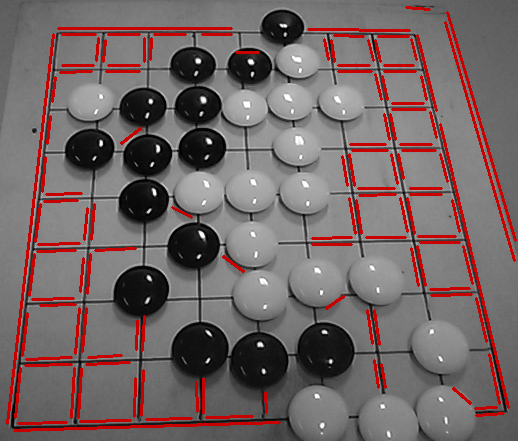
\includegraphics[width=0.45\columnwidth]{images/lsd_length.png}
					\end{subfigure}
					\\
					\begin{subfigure}{}
						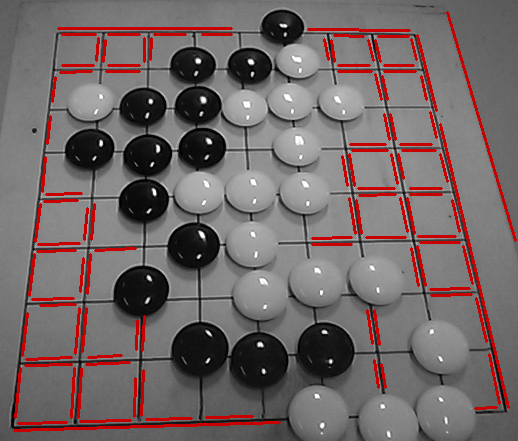
\includegraphics[width=0.45\columnwidth]{images/lsd_parallel.png}
					\end{subfigure}
					\begin{subfigure}{}
						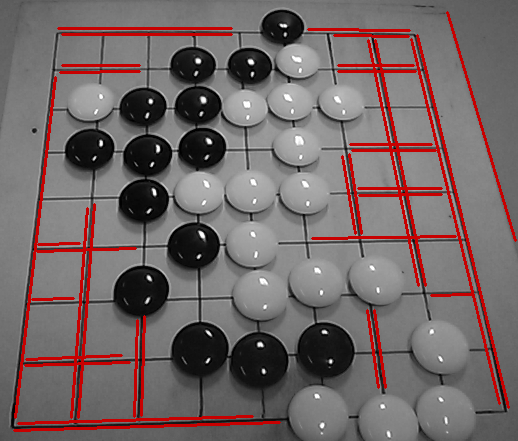
\includegraphics[width=0.45\columnwidth]{images/lsd_final.png}
					\end{subfigure}
				\end{center}
			\end{figure}
		\end{column}
	\end{columns}
\end{frame}

\subsection{Detection of Pieces}
\begin{frame}{Detection of Pieces}{Thresholding}
	\begin{columns}
		\begin{column}{0.6\textwidth}
			To segment the tokens from the background we use thresholding\\[0.5cm]

			White pieces are a problem due to color aberration\\
			$\Rightarrow$ Threshold in HSV space, use combined results from saturation and hue channel\\[0.5cm]

			To detect the pieces we use \emph{Hough Transformation} or fit rectangles around the blobs and filter for squares
		\end{column}
		\begin{column}{0.3\textwidth}
			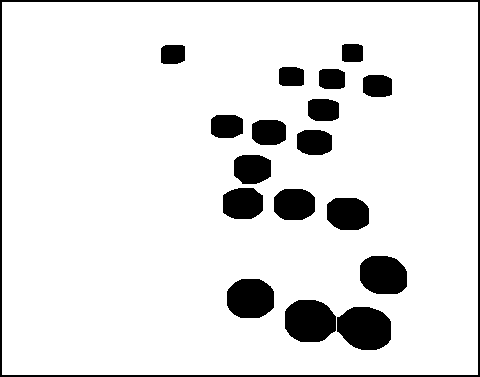
\includegraphics[width=\columnwidth]{images/pieces_thresh_s.png}\\
			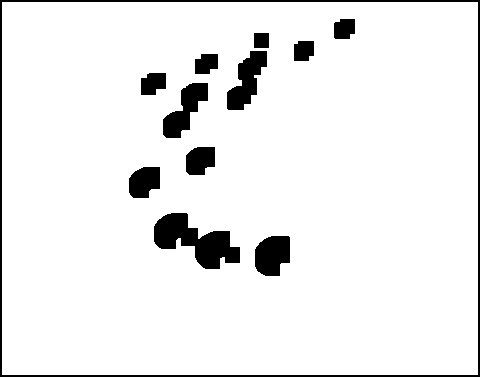
\includegraphics[width=\columnwidth]{images/pieces_thresh_v.png}
		\end{column}
	\end{columns}
\end{frame}
% \begin{frame}{Detection of Pieces}{using Hough Circle Transformation}~\end{frame}
% \begin{frame}{Detection of Pieces}{using contours of pieces}~\end{frame}

\subsection{Extrapolating the Board}
\begin{frame}{Extrapolating the Board}
	\begin{columns}
		\begin{column}{0.6\textwidth}
			We finally fill the intersections by
			\begin{itemize}
				\item rotating intersections to be horizontal
				\item selecting 20 around the center
				\item building a model from them
				\item detecting orientation of model with RANSAC
				\item using orientation to extrapolate board
				\item using detected intersections to refine extrapolation
			\end{itemize}
		\end{column}
		\begin{column}{0.3\textwidth}
			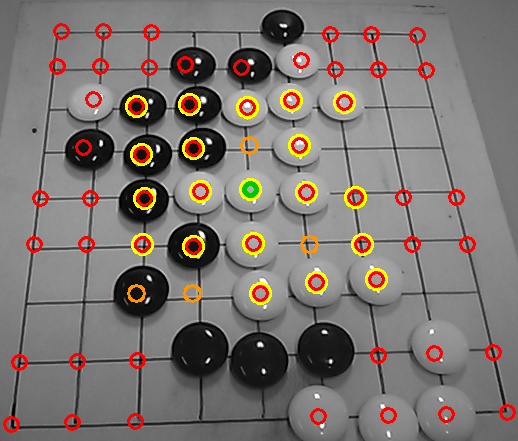
\includegraphics[width=\columnwidth]{images/buildingModel.png}\\
			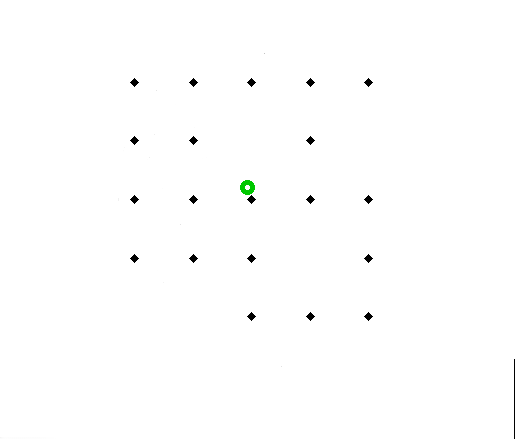
\includegraphics[width=\columnwidth]{images/builtModel.png}
		\end{column}
	\end{columns}
\end{frame}
\subsection{Postprocessing}
\begin{frame}{Postprocessing}
	We try to filter out invalid detection results. We consider results invalid if one intersection is
	\begin{itemize}
		\item outside the image
		\item or closer than 5px to each other.
	\end{itemize}
	\vspace{0.5cm}

	We undo the cropping from the preprocessing step.\\[0.5cm]

	We smooth results over time: only if a token was detected in 5 of the last 10 frames we count it as accurate.
\end{frame}

\section{Evaluation}
\frame[squeeze]{\tableofcontents[currentsection]}
\subsection{Detection Quality}
\begin{frame}{Detection Quality}~\end{frame}
\subsection{Speed}
\begin{frame}{Speed}~\end{frame}

\section{Conclusion}
\subsection{Our Contribution}
\begin{frame}{Our Contribution}~\end{frame}
\subsection{Future Work}
\begin{frame}{Future Work}~ \end{frame}
\subsection{Live Presentation?}
\begin{frame}{Live presentation}{Because seeing is believing}\end{frame}

\section*{Questions}
\centering
\begin{frame}
  \huge Thank you for your attention.\\[1.5cm] Questions?
\end{frame}

\end{document}
\endinput
%%
%% End of file `01-example'.
